\subsection{Comportamento dinamico}

Fino ad ora abbiamo caratterizzato lo ShuntLDO a $2 \A$ con carico statico.
\`E per\`o fondamentale studiare il comportamento dello ShuntLDO in risposta ad una variazione dinamica del carico, focalizzando l'attenzione sulla velocità dello shunt nel riequilibrare il consumo in corrente. 
%Fino ad ora abbiamo studiato la caratterizzazione dello ShuntLDO a $2\A$ con carichi statici in condizioni stazionarie.
%Oltre alla caratterizzazione statica un punto fondamentale è studiare il comportamento dello ShuntLDO in risposta ad una variazione dinamica del carico, andando a focalizzare l'attenzione sulla velocità dello shunt nel riequilibrare il consumo in corrente. 
%La risposta dinamica dipende da molti fattori quali: il punto di lavoro dello ShuntLDO, i tempi caratteristici della variazione di carico e l'entità di tale variazione. 
La risposta dinamica dipende da molti fattori tra cui: il punto di lavoro a cui si trova lo ShuntLDO, il tempo in cui avviene la variazione di carico e l'entità di tale variazione.

Per effettuare i test si è alimentato il circuito tramite un generatore di corrente a $1.5 \A$, ponendo la tensione di riferimento $\mathrm{V_{ref}=0.5 \A}$. %, ci aspettiamo una tensione all'uscita di $1 \V$.
Sulla scheda di test, per dare la possibilità di introdurre un carico dinamico, è presente un mosfet in serie ad una resistenza, R5, di $0.1 \Omega$, che è posto in parallelo al carico statico, $\mathrm{R_{load}}$, tramite l'impiego di un opportuno {\em jumper}.
La corrente assorbita dal mosfet, indicata con $\mathrm{I_{mosfet}}$, può essere calcolata, misurando la caduta di tensione su R5, e regolata, pilotando la tensione applicata al gate, ad esempio utilizzando, come nel caso dei test effettuati, un generatore di impulsi esterno.
%Il circuito è alimentato tramite un generatore di corrente a $1.5 \A$ e la tensione di riferimento per $\mathrm{V_{out}}$ è posta pari a $\mathrm{V_{ref}=0.5 \A}$.%, ci aspettiamo una tensione all'uscita di $1 \V$.
%Al fine di introdurre un carico dinamico, in parallelo al carico statico, è presente sulla scheda di test un mosfet in serie ad una resistenza, R5, di $0.1 \Omega$.
%La corrente assorbita dal mosfet, indicata con $\mathrm{I_{mosfet}}$, può essere calcolata misurando la caduta di tensione su R5 ed è regolabile attraverso la tensione applicata al gate, in questo caso collegato ad un generatore di impulsi esterno.
%A seconda dell'ampiezza del segnale inviato al Gate del mosfet si avrà una maggiore o minore corrente che scorre tra Drain e Source. 
Il setup di queste misure è rappresentato schematicamente in Fig.~\ref{Setupscheme}.
%: sulla sinistra in verde, la scheda di test; in grigio sono riportati gli alimentatori; sulla destra l'oscilloscopio con cui sono misurate la tensione in ingresso $\mathrm{V_{in}}$
%\footnote{
%L'alimentazione dello ShuntLDO è comunque in corrente.
%}, rappresentata in giallo, la tensione in uscita $\mathrm{V_{out}}$, in arancione, e le tensioni agli estremi della resistenza R5 in azzurro; infine, sulla sinistra della scheda di test, collegato al gate del mosfet, è presente un generatore di impulsi. 
La durata dell'impulso da mandare al Gate del mosfet è stata scelta tale da mantenere fronte di salita e discesa indipendenti, in modo da osservare separatamente gli effetti dovuti all'uno e all'altro.
%Infatti, in una situazione in cui il carico del regolatore è il chip le variazioni sarebbero di minor durata rispetto alla lunghezza dell'impulso utilizzato in queste misure.
Inoltre, lo scopo delle misure è di vedere gli effetti del passaggio da un certo consumo di corrente ad uno maggiore (e viceversa) e l'utilizzo di un impulso di breve durata sovrapporrebbe i due effetti, non permettendo di valutarli correttamente, poiché, essendo opposti, su tempi brevi si cancellerebbero a vicenda.
%Ad ogni modo lo scopo di queste misure è quello di vedere gli effetti al passaggio da un certo consumo di corrente ad uno maggiore e viceversa ed un impulso di breve durata sovrapporrebbe questi due effetti, non permettendo di valutarli correttamente, in quanto i contributi sono opposti e, su tempi brevi, si cancellerebbero a vicenda.
In queste misure l'attenzione sarà focalizzata sulle variazioni in ampiezza di $\mathrm{V_{in}}$ e $\mathrm{V_{out}}$ e sul tempo di recupero di queste, in funzione di $\mathrm{I_{mosfet}}$ e con $\mathrm{R_{load}}$ fissata.
%In queste misure l'attenzione sarà focalizzata su variazioni di $\mathrm{V_{in}}$ e $\mathrm{V_{out}}$ in ampiezza e sul tempo di recupero al variare di $\mathrm{I_{mosfet}}$ per una data $\mathrm{R_{load}}$.
\begin{figure}[!htb]
\centering
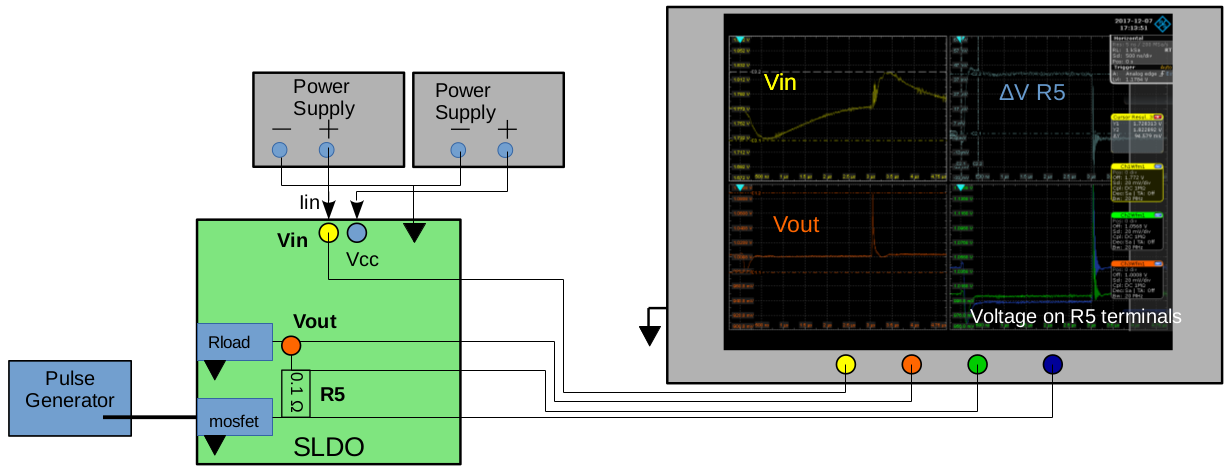
\includegraphics[scale=.3]{Immagini/SetupScheme}
\caption{Schema del setup per lo studio del comportamento dinamico dello ShuntLDO. In grigio sono riportati gli alimentatori e in verde è rappresentata la scheda di test su cui, in azzurro, sono evidenziati mosfet e carico resistivo. Collegato al Gate del mosfet, sulla sinistra, vi è l'impulsatore. Sulla destra è rappresentato l'oscilloscopio attraverso cui sono monitorate le tensioni di ingresso $\mathrm{V_{in}}$, di uscita $\mathrm{V_{out}}$ e quelle ai capi di R5.}
%\caption{Schema del setup per lo studio del comportamento dinamico dello ShuntLDO. In grigio sono riportati gli alimentatori e in verde è rappresentata la scheda di test su cui in azzurro sono evidenziati mosfet e carico resistivo, collegato al Gate del mosfet, sulla sinistra, vi è l'impulsatore. Infine, sulla destra è rappresentato l'oscilloscopio attraverso cui sono monitorate le tensioni di ingresso $\mathrm{V_{in}}$, di uscita $\mathrm{V_{out}}$ e quelle ai capi di R5.}
\label{Setupscheme}
\end{figure}

%L'introduzione del carico $\mathrm{R_{load}}$ in parallelo alla resistenza connessa a $\mathrm{V_{out}}$ è possibile andando a modificare la configurazione della scheda di test.
Fin dalle prime misure con l'oscilloscopio è possibile notare che l'utilizzo del mosfet come carico dinamico non è esente da fenomeni di alterazione dei segnali, rendendo difficile una loro corretta interpretazione.
%Dalle prime misure con l'oscilloscopio è possibile vedere che che l'utilizzo del mosfet come carico dinamico non è esente da fenomeni di alterazione dei segnali, ciò rende difficile una loro corretta interpretazione. 
\begin{figure}
\begin{subfigure}{.5\textwidth}
  \centering
  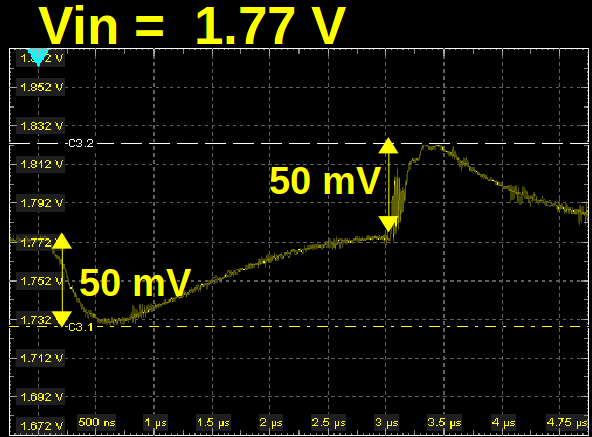
\includegraphics[width=.96\linewidth]{Immagini/zoomTransientTest1}
  \caption{ }
  \label{TransientTest:sfig1}
\end{subfigure}%
\begin{subfigure}{.5\textwidth}
  \centering
  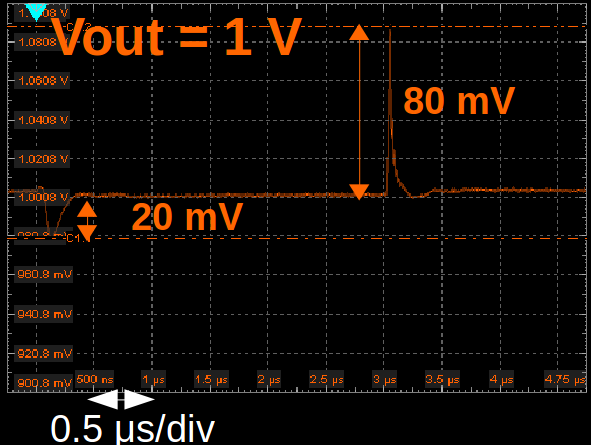
\includegraphics[width=.95\linewidth]{Immagini/zoomTransientTest2}
  \caption{ }
  \label{TransientTest:sfig2}
\end{subfigure}
\begin{subfigure}{\textwidth}
  \centering
  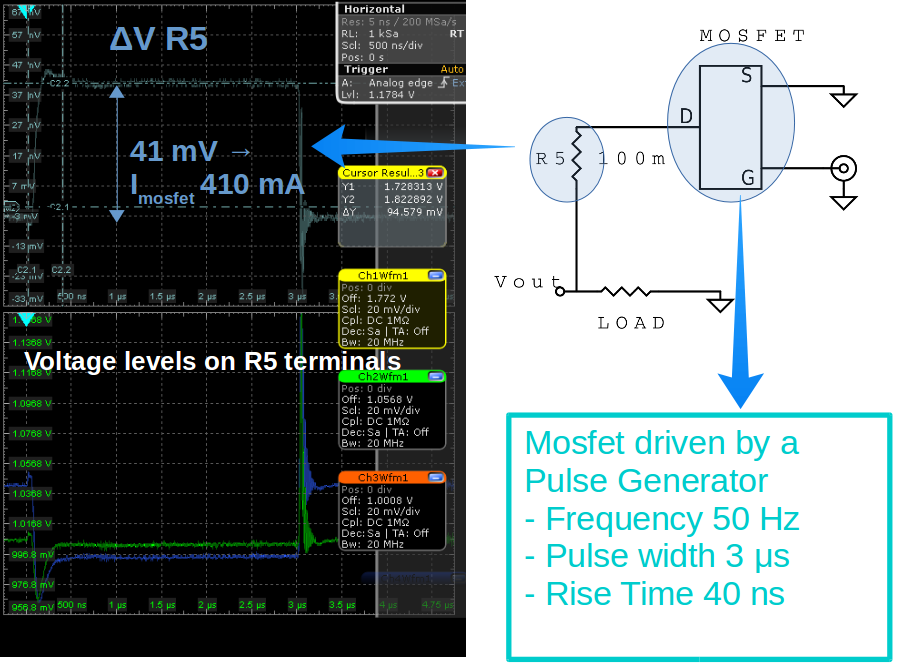
\includegraphics[width=0.9\linewidth]{Immagini/zoomTransientTest3bis}
  \caption{ }
  \label{TransientTest:sfig3}
\end{subfigure}
\caption{Schermata catturata dall'oscilloscopio: in giallo è rappresentata la tensione in ingresso, in arancione quella in uscita e in verde e blu la tensione sui i terminali di R5, la cui differenza è riportata in  azzurro. Nella sottofigura~\ref{TransientTest:sfig3}, a lato della schermata dell'oscilloscopio, è riportato lo schematico della parte di circuito con mosfet e resistenza.}
\label{TransientTest}
\end{figure}
Prendendo come riferimento la Fig.~\ref{TransientTest}, infatti, si può notare un'asimmetria nelle variazioni di $\mathrm{V_{out}}$, riportato in arancione nel grafico in alto a destra. %, mentre in $\mathrm{V_{in}}$, in giallo in alto a sinistra, la risposta è simmetrica.
%Prendendo come riferimento la figura \ref{TransientTest}, si può notare un'asimmetria nelle variazioni di $\mathrm{V_{out}}$, in arancione in alto a destra.%, mentre in $\mathrm{V_{in}}$, in giallo in alto a sinistra, la risposta è simmetrica.
Allo stesso modo nella sottofigura~\ref{TransientTest:sfig3} in azzurro, è riportata la differenza tra le tensioni misurate ai capi di R5 (in blu e verde nel grafico in basso) e in cui si vede un'asimmetria in risposta al fronte di salita e discesa dell'impulso applicato al Gate del mosfet.
%Allo stesso modo nella sottofigura~\ref{TransientTest:sfig3} in azzurro, è riportata la differenza tra le tensioni misurate ai capi di R5, riportate in basso con colore blu e verde e in cui si vede un'asimmetria in risposta al fronte di salita e discesa dell'impulso applicato al Gate del mosfet. 
Inoltre, sono visibili delle oscillazioni in corrispondenza dell'istante in cui il mosfet si spegne, sia sulle tensioni riferite a R5 sia sul $\mathrm{V_{out}}$.
%Questo comportamento si riflette su $\mathrm{V_{out}}$ ed è quindi all'origine dell'asimmetria.
Prima di procedere con misure dinamiche nelle varie combinazioni $\mathrm{I_{mosfet}}$--$\mathrm{R_{load}}$ si è cercato di capire l'origine delle asimmetria, in particolare chiedendosi se dipende dalla risposta del mosfet all'impulso sul Gate.
%Prima di procedere con misure dinamiche nelle varie combinazioni $\mathrm{I_{mosfet}}$--$\mathrm{R_{load}}$ si è cercato di capire l'origine delle asimmetria, in particolare se fosse collegata alla risposta del mosfet all'impulso.
L'impulso utilizzato in questa prima fase ha:
\begin{itemize}
  \item frequenza di $50\Hz$;
  \item durata di 3 $\mu$s;
  \item fronte di salita di $40 \ns$.
\end{itemize}
%In questa prima fase l'impulso utilizzato ha le seguenti caratteristiche: frequenza 50 Hz, durata 3 $\mu$s, durata del fronte di salita 40 ns.

\subsubsection{Contributo mosfet}
\begin{figure}
\centering
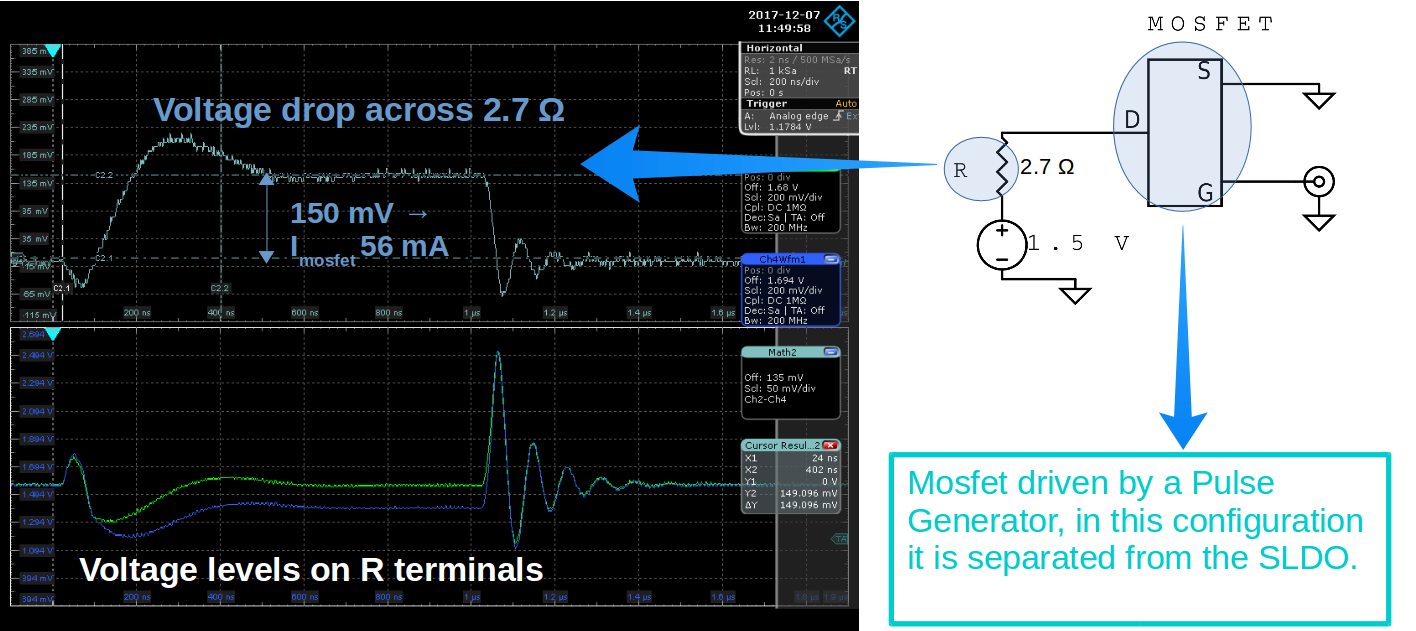
\includegraphics[width=\linewidth]{Immagini/MosfetBehaviourbis}
\caption{Sulla sinistra è riportato la schermata dell'oscilloscopio, che mostra l'andamento della tensione sui terminali di R in funzione del tempo, sulla destra è invece riportato lo schema della modifica al circuito.}
\label{MosfetBehaviour}
\end{figure}

\begin{figure}
\centering
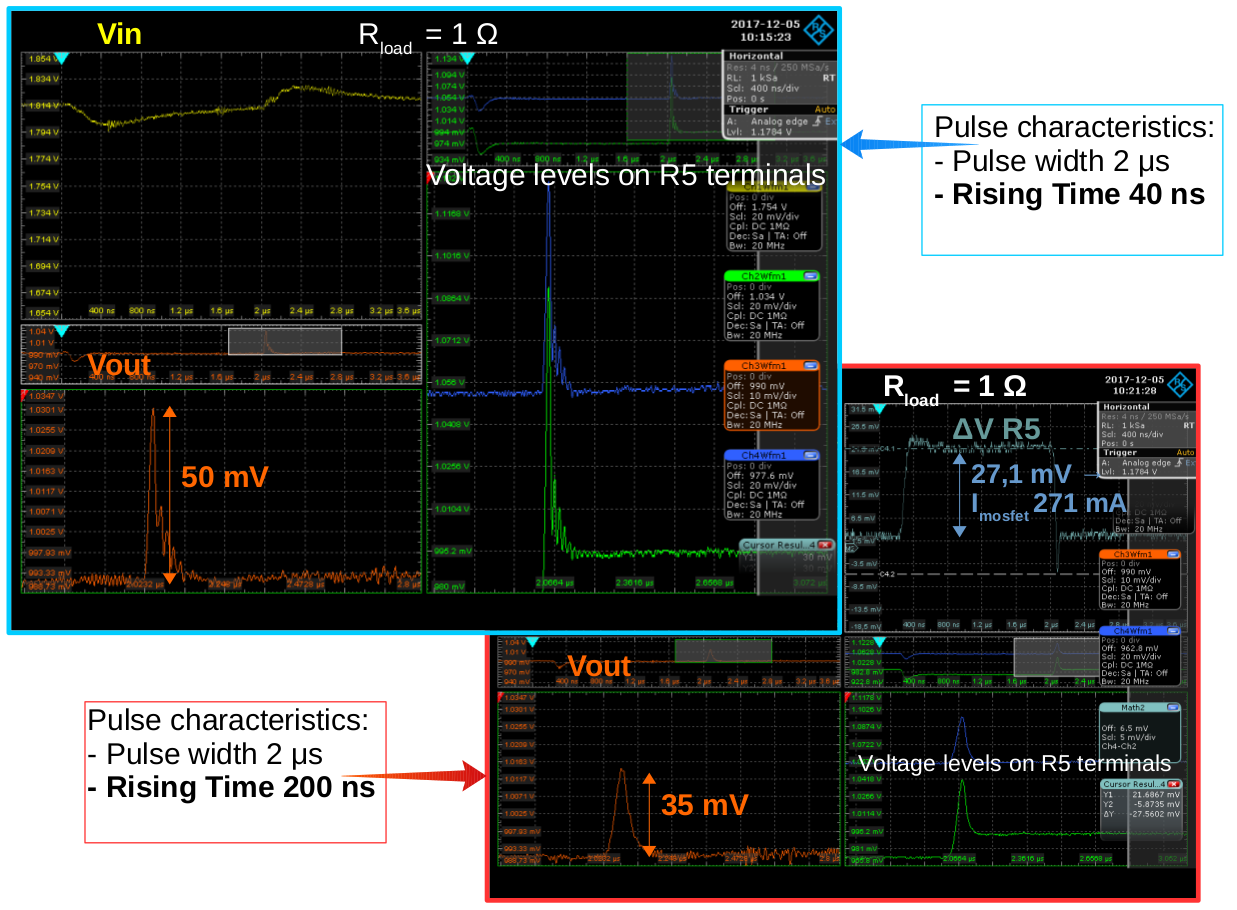
\includegraphics[width=\linewidth]{Immagini/RiseTime}
\caption{In alto a sinistra è riportata la risposta del $\mathrm{V_{out}}$ per impulsi con tempo di salita 40 ns, il basso a destra invece è la risposta a impulsi con tempi di salita di 200ns. Sia per il $\mathrm{V_{out}}$ che per le tensioni su R5 il comportamento migliora rallentando l'impulso.}
\label{RiseTime}
\end{figure}

Per esaminare il comportamento del mosfet in risposta all'impulso mandato sul Gate, si è realizzato un allestimento di test specifico, mostrato nella parte a destra della Fig.~\ref{MosfetBehaviour}: il Drain del mosfet è stato disconnesso dal resto del circuito del chip e connesso ad una batteria stilo esterna, che ricopre il ruolo di $\mathrm{V_{out}}$, con in serie una resistenza di 2.7 $\Omega$, utilizzata per misurare le correnti che sorrono nel mosfet.
%Per esaminare il comportamento del mosfet in risposta all'impulso mandato sul Gate, si è proceduto ad isolare questa parte del circuito dal resto della scheda di test, connettendo al Drain una resistenza in serie ad una batteria stilo, al posto della connessione con il $\mathrm{V_{out}}$ dello ShuntLDO.
%La batteria ricopre il ruolo di $\mathrm{V_{out}}$, mentre la resistenza è necessaria alla misura delle correnti che scorrono nel mosfet ed ha un valore di 2.7 $\Omega$. 

La Fig.~\ref{MosfetBehaviour} a sinistra, mostra la caduta di tensione ai capi della resistenza in serie alla batteria: le oscillazioni già osservate con il chip connesso e presenti in corrispondenza dello spegnimento del mosfet, sono evidenti anche con questo allestimento.
Esse sono, dunque, generate dal mosfet stesso nel momento in cui il canale, che collega Drain e Source, si interrompe e non dipendono da $\mathrm{V_{out}}$.
Inoltre, il fronte di salita è circa $100 \ns$, più lungo di quello dell'impulso, indice del fatto che il mosfet ha una risposta più lenta. %e non $40 \ns$ come ci aspetteremmo da un mosfet ideale con risposta istantanea.
Esaminando la documentazione del mosfet~\cite{MOSFET} presente sulla scheda di test 
%footnote{ZXMN20B28KTC http://www.mouser.com/ds/2/115/ZXMN20B28K-94822.pdf
si può verificare che effettivamente il tempo di ``accensione'' è superiore a $40 \ns$ (\textit{Turn-on rise time} $76.9 \ns$) e, inoltre, sono presenti capacità in ingresso equivalenti a $358\pF$.
La risposta dello ShuntLDO è quindi mascherata per segnali più veloci della risposta del mosfet, per questo motivo le misure successive sono state effettuate utilizzando un tempo di salita del segnale del generatore di impulsi di $200 \ns$.
La Fig.~\ref{RiseTime} mostra il miglioramento fra la configurazione con tempo di salita del generatore di $40 \ns$ e quella con $200 \ns$.
In questo modo si verifica la risposta dello ShuntLDO cad una variazione di carico più lenta, ma meno affetta dal mosfet.
%In figura \ref{RiseTime} è visibile come la situazione precedente, in cui l'impulso ha un tempo di salita di 40 ns, migliora visibilmente passando a 200 ns, in questo modo quello che viene simulato all'uscita dello ShuntLDO è un variazione di carico più lenta ma il cui comportamento è affetto in modo minore dalle caratteristiche del mosfet. 

\subsubsection{Misure}

Di seguito sono riportate le misure di caratterizzazione della tensione di ingresso, $\mathrm{V_{in}}$, e di uscita, $\mathrm{V_{out}}$, per tre differenti valori di $\mathrm{R_{load}}$ e al variare di $\mathrm{I_{mosfet}}$.
I valori di $\mathrm{R_{load}}$ scelti sono: $1 \Ohm$, $2.1 \Ohm$ e $4 \Ohm$; dato che $\mathrm{V_{out}=1 \V}$, in termini di correnti  $\mathrm{I_{load}}$, questi corrispondono rispettivamente a $1 \A$, $0.475 \A$ e $0.250 \A$.
%Oltre alla misura delle variazioni in ampiezza di $\mathrm{V_{in}}$ e $\mathrm{V_{out}}$ sono stati misurati anche i tempi di  recupero delle stesse.

\`E interessante notare che il tempo di recupero di $\mathrm{V_{in}}$ e $\mathrm{V_{out}}$ differiscono notevolmente: il primo è molto più lungo, dell'ordine dei $\mu$s, e dipendente dal valore di $\mathrm{I_{mosfet}}$, il secondo ha durata di circa $300 \ns$ indipendentemente dal valore di $\mathrm{I_{mosfet}}$.
Questo comportamento è imputabile al fatto che il riequilibrio della tensione di ingresso dipende anche dal generatore esterno, le cui variazioni sono più lente.
Va ricordato che lo ShuntLDO è alimentato in corrente con $1.5 \A$, dunque nel momento in cui $\mathrm{I_{load}+I_{mosfet}}$ raggiungono valori vicini o addirittura superiori  a $\mathrm{I_{in}}$, si ha un crollo della tensione in ingresso e del $\mathrm{V_{out}}$, poiché si sta chiedendo allo ShuntLDO di fornire una corrente superiore a quella a sua disposizione.

Per ciascun valore di $\mathrm{R_{load}}$, dunque, è stata fatta variare la corrente assorbita dal mosfet $\mathrm{I_{mosfet}}$ e misurato l'effetto di undershoot e overshoot sulle tensioni di $\mathrm{V_{out}}$ e $\mathrm{V_{in}}$. 
% Con corrente totale si intende la somma di quella assorbita dal mosfet e dalla resistenza di carico.
Le misure eseguite prendono in considerazione anche situazioni in cui la variazione del consumo in corrente eccede l'intervallo fisico di operatività del chip. Misure in cui la variazione del carico è il doppio del valore statico hanno interesse nell'ottica di quello che può succedere al momento dell'accensione del ROC. %, le cui variazioni di consumo in regime di lavoro, di norma, non superano i 500 mA.(controllare) 
Come detto in precedenza, gli impulsi utilizzati presentano una durata che consente di differenziare tra gli effetti dovuti al fronte di salita e quelli prodotti dal fronte di discesa. 
Facendo riferimento alla Fig.~\ref{VoutUnd}, si possono vedere, in valore assoluto,gli undershoot della tensione di uscita a cui è applicato il carico in funzione della corrente che scorre nel mosfet (sinistra) e della corrente totale (destra), dove questa è la somma di quella assorbita dal carico e quella del mosfet. 
%I primi risultati riportano gli undershoot della tensione di uscita a cui è applicato il carico, riferendosi ai grafici in Fig.~\ref{VoutUnd} sono riportati i valori assoluti di tali variazioni in funzione della corrente che scorre nel mosfet (sinistra) e della corrente totale (destra), la corrente totale è somma di quella assorbita dal carico e dal mosfet. 
\begin{figure}
\centering
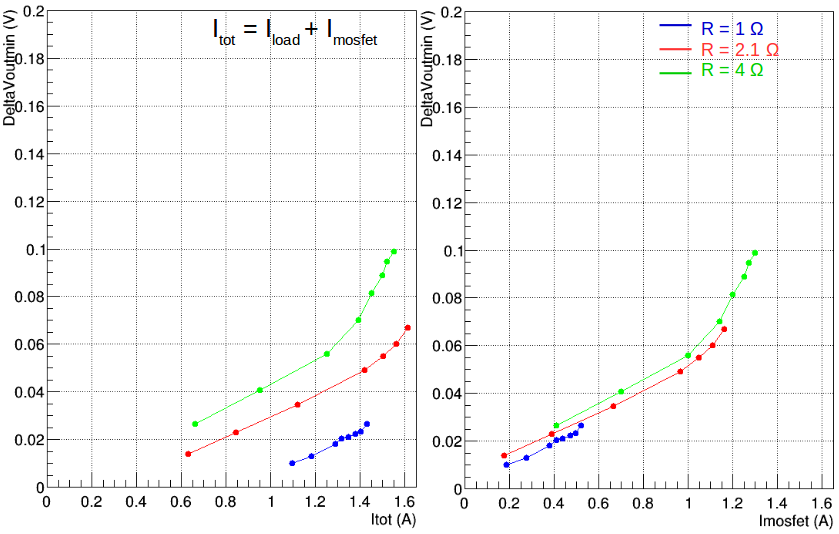
\includegraphics[width=0.9\linewidth]{Immagini/VoutUnd}
\caption{Grafici che riportano l'entità dell'undershoot del $\mathrm{V_{out}}$ in funzione della corrente totale, grafico di sinistra, e della corrente del mosfet, grafico di destra.}
\label{VoutUnd}
\end{figure}
\begin{figure}
\centering
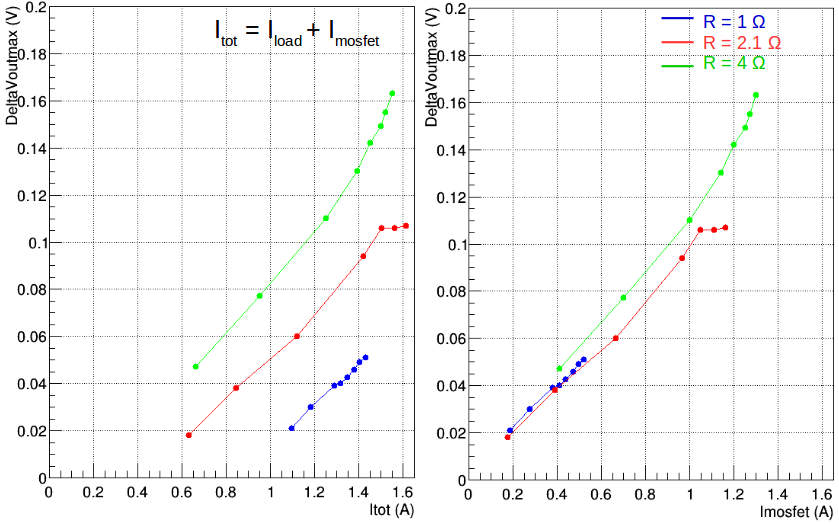
\includegraphics[width=0.9\linewidth]{Immagini/VoutOver}
\caption{Grafici che riportano l'entità dell'overshoot del $\mathrm{V_{out}}$ in funzione della corrente totale, grafico di sinistra, e della corrente del mosfet, grafico di destra.}
\label{VoutOver}
\end{figure}
In blu sono riportate le misure ottenute con un carico resistivo di $1 \Ohm$, in rosso $2.1 \Ohm$  e in verde $4 \Ohm$.
Come si può vedere dal grafico di destra, le tre curve seguono lo stesso andamento, dato che vi è una relazione fra la variazione di $\mathrm{V_{out}}$ e $\mathrm{I_{mosfet}}$, indipendente dal valore della resistenza.
Inoltre, limitandosi ad un intervallo di variazioni di corrente verosimili per il ROC, si osservano variazioni relativamente piccole di $\mathrm{V_{out}}$.
Ad esempio, con $\mathrm{I_{mosfet}= 0.4 \A}$, $\mathrm{\Delta V_{out} \simeq 20\mV}$.
Lo stesso comportamento è visibile nei grafici di Fig.~\ref{VoutOver}, dove è riportata l'entità delle variazioni di $\mathrm{V_{out}}$ a seguito dello spegnimento del mosfet, cioè l'effetto che si ha sul fronte di discesa dell'impulso. 
%Nell'esaminare questi andamenti va ricordato che la corrente in ingresso al circuito è 1.5 A, quindi punti per i quali si ha una $\mathrm{I_{tot}}$ vicina o superiore a questo valore sono ottenuti in una situazione in cui lo ShuntLDO è impossibilitato a compiere il suo lavoro. 
%Ricordiamo che la corrente che passa in $R_3$ è un millesimo di quella che scorre nel ramo in cui si hanno carico e shunt.

Come per il $\mathrm{V_{out}}$ è stato misurato l'undershoot e l'overshoot della tensione in ingresso $\mathrm{V_{in}}$. I grafici degli undershoot sono riportati in Fig.~\ref{VinUnd}, quelli riguardanti gli overshoot in Fig.~\ref{VinOver}. 

\begin{figure}
\centering
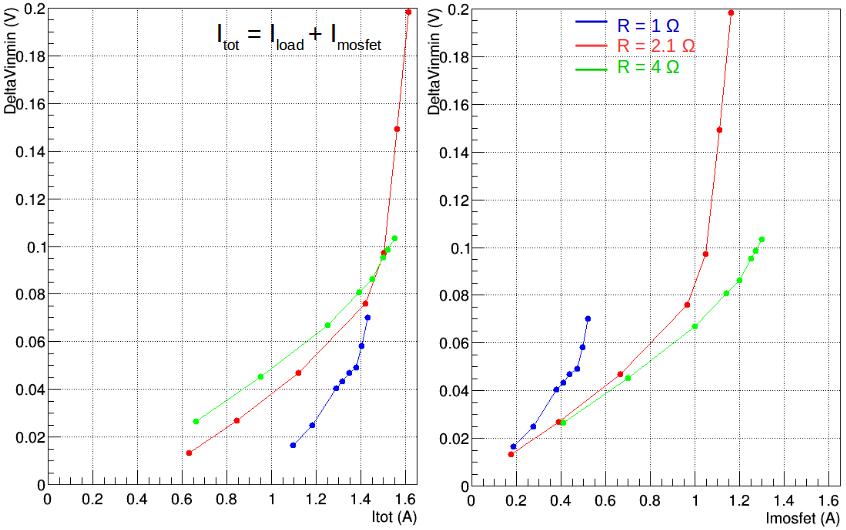
\includegraphics[width=0.9\linewidth]{Immagini/VinUnd}
\caption{Grafici che riportano l'entità dell'undershoot del $\mathrm{V_{in}}$ in funzione della corrente totale, grafico di sinistra, e della corrente del mosfet, grafico di destra.}
\label{VinUnd}
\end{figure}

\begin{figure}
\centering
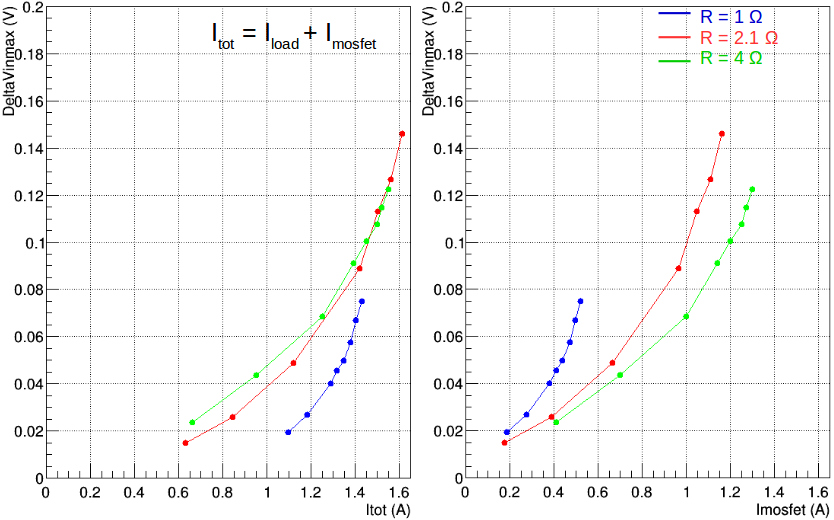
\includegraphics[width=0.9\linewidth]{Immagini/VinOver}
\caption{Grafici che riportano l'entità dell'undershoot del $\mathrm{V_{in}}$ in funzione della corrente totale, grafico di sinistra, e della corrente del mosfet, grafico di destra.}
\label{VinOver}
\end{figure}

In entrambi i casi la variazione della tensione in ingresso dipende sia dalla variazione di corrente $\mathrm{I_{mosfet}}$ che dalla corrente fissa $\mathrm{I_{load}}$. 
Per valori elevati di $\mathrm{I_{mosfet}}$ la tensione in ingresso inizia ad oscillare, con periodi di qualche $\mu$s.
Questo comportamento è dovuto al generatore utilizzato, in particolare l'alimentazione in corrente è stata ottenuta utilizzando un generatore di tensione, ma limitando la corrente in uscita. 
Nel momento in cui si ha una variazione di carico molto veloce che provoca un abbassamento di $\mathrm{V_{out}}$, si ha una piccola ripercussione sulla tensione di ingresso: dato che il generatore è di tensione, limitato in corrente, per tenere costante $\mathrm{I_{in}}$ avrà un abbassamento di tensione, ma con tempi più lunghi rispetto a quelli con cui lo ShuntLDO riesce a riequilibrare $\mathrm{V_{out}}$.
Il comportamento oscillatorio di $\mathrm{V_{in}}$, che compare quando $\mathrm{I_{tot}}$ è intorno al valore massimo, $\mathrm{I_{in}}$, ha permesso di constatare come fluttuazioni della tensione in ingresso non influiscano sulla tensione generata dal regolatore.
Questo può essere visto utilizzando l'oscilloscopio: in Fig.\ref{DipVoutVin} è mostrata una schermata dell'oscilloscopio in cui è riportato, in giallo, l'andamento di $\mathrm{V_{in}}$ in funzione del tempo, e, in arancione, la tensione di $\mathrm{V_{out}}$.
Si nota che le scale di tempo di recupero sono differenti, i.e. alcuni $\mu$s per $\mathrm{V_{in}}$ e circa $300 \ns$ per $\mathrm{V_{out}}$.

\begin{figure}
\begin{subfigure}{.5\textwidth}
  \centering
  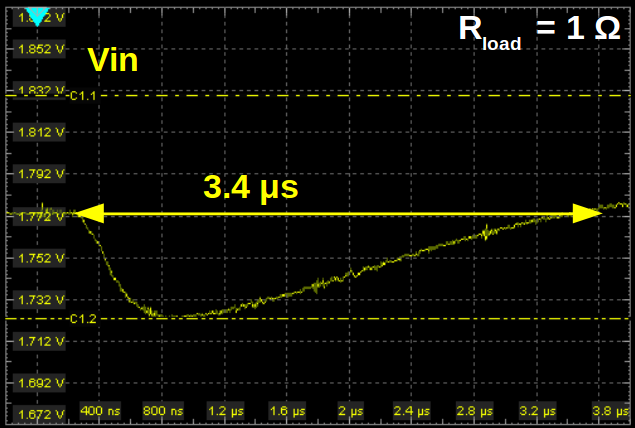
\includegraphics[width=.95\linewidth]{Immagini/zoomDipendenzaVoutdaVin1}
  \caption{1a}
  \label{DipVoutVin:sfig1}
\end{subfigure}%
\begin{subfigure}{.5\textwidth}
  \centering
  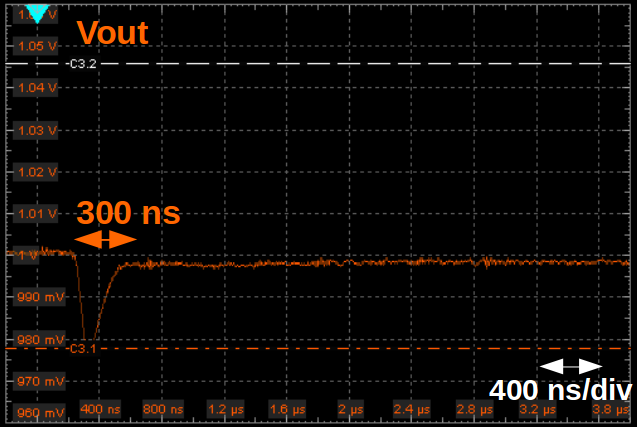
\includegraphics[width=.95\linewidth]{Immagini/zoomDipendenzaVoutdaVin2}
  \caption{1b}
  \label{DipVoutVin:sfig2}
\end{subfigure}
\caption{Differenze nei tempi di recupero tra $\mathrm{V_{out}}$, in giallo, e $\mathrm{V_{out}}$, in arancione.}
\label{DipVoutVin}
\end{figure}
%\begin{figure}
%\centering
%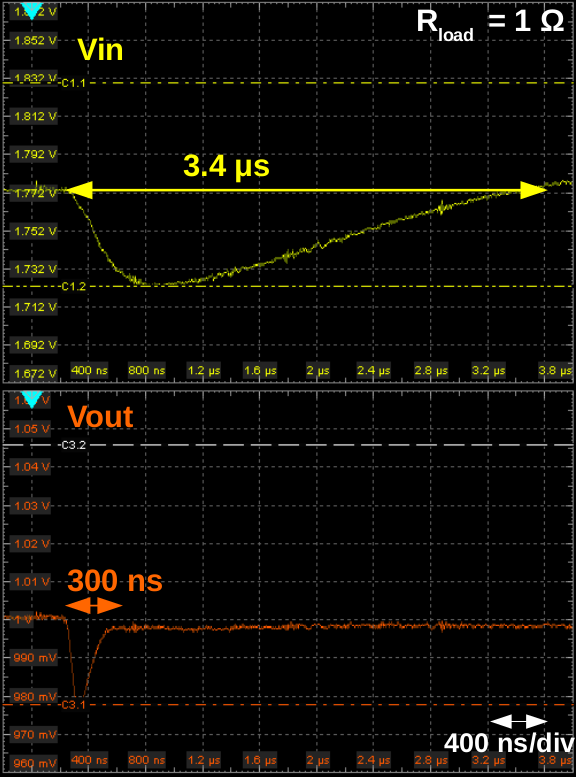
\includegraphics[scale=.35]{Immagini/DipendenzaVoutdaVin}
%\caption{Differenze nei tempi di recupero tra $\mathrm{V_{out}}$, in giallo, e $\mathrm{V_{out}}$, in arancione.}
%\label{DipVoutVin}
%\end{figure}

\subsubsection{Serie di due ShuntLDO}

Dato che eventuali oscillazioni della tensione in ingresso causerebbero oscillazioni di tensione in tutta la catena di moduli, è importante che queste non si ripercuotano sul $\mathrm{V_{out}}$. 
Per verificare questo aspetto si è misurato con l'oscilloscopio la tensione di uscita di uno ShuntLDO messo in serie ad un secondo a cui è applicato un carico variabile, tramite l'utilizzo del mosfet, come già visto nelle misure precedenti.
In Fig.~\ref{SLDOserie} sono affiancati uno schema del setup (sinistra) e la foto dei due ShuntLDO in serie (destra). 
Il serie di due ShuntLDO, entrambi con un carico statico di $4 \Ohm$, è alimentato con una corrente in ingresso di $1.5 \A$ e sul secondo ShuntLDO è collegato l'impulsatore che regola l'assorbimento di corrente  da parte del mosfet. 
Acquisendo con l'oscilloscopio la tensione di $\mathrm{V_{out}}$ di entrambi e il $\mathrm{V_{in}}$ del primo ShuntLDO della catena (quello con il solo carico statico) è stato possibile verificare come le fluttuazioni di tensione non influenzino la generazione della tensione di $\mathrm{V_{out}}$.
\begin{figure}[h!]
\centering
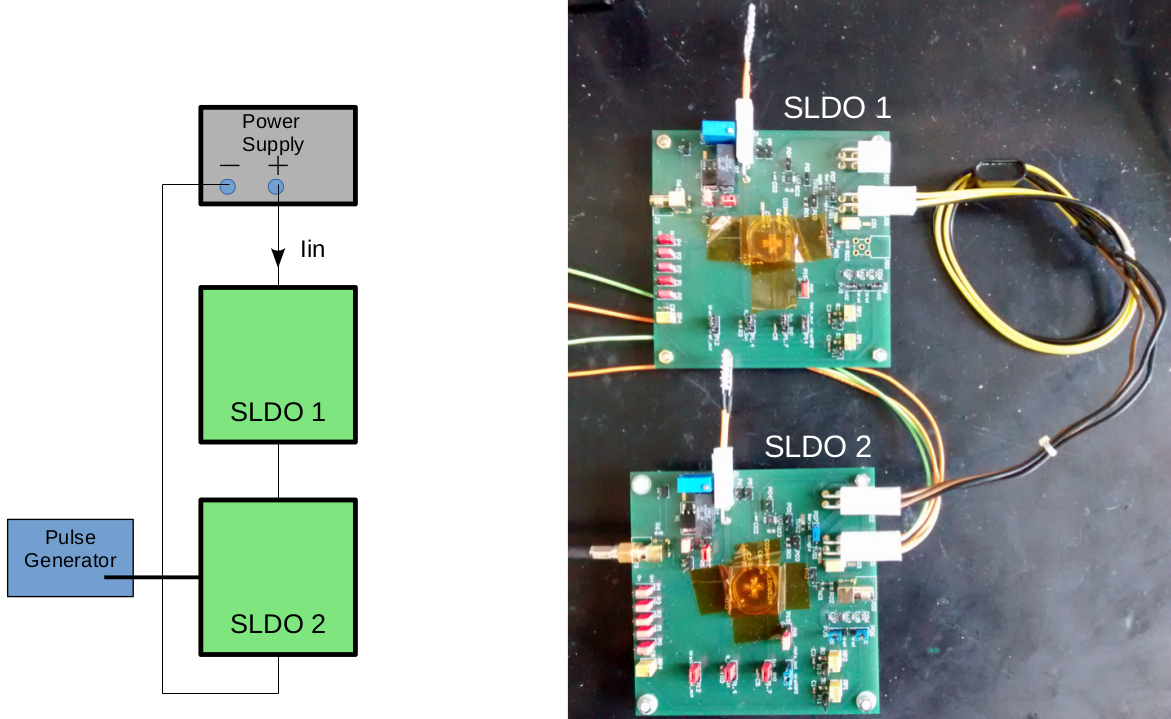
\includegraphics[scale=.30]{Immagini/SLDOserie}
\caption{Sulla destra foto dei due ShuntLDO in serie di cui a sinistra è riportato uno schema delle connessioni con generatore e impulsatore.}
\label{SLDOserie}
\end{figure}
In particolare in Fig.~\ref{ScreenSerie} si vede che, nonostante il secondo ShuntLDO sia in una situazione estrema, la generazione di $\mathrm{V_{out}}$ da parte del primo non ha ripercussioni. 
Il campionamento dei segnali mostrati, acquisiti con l'oscilloscopio, è stato ottenuto con una $\mathrm{I_{mosfet}}$ di $1.2 \A$, corrispondenti ad una $\mathrm{I_{tot}}$ di circa $1.45 \A$, quindi molto vicino al limite di $1.5 \A$. 
\begin{figure}[h!]
\centering
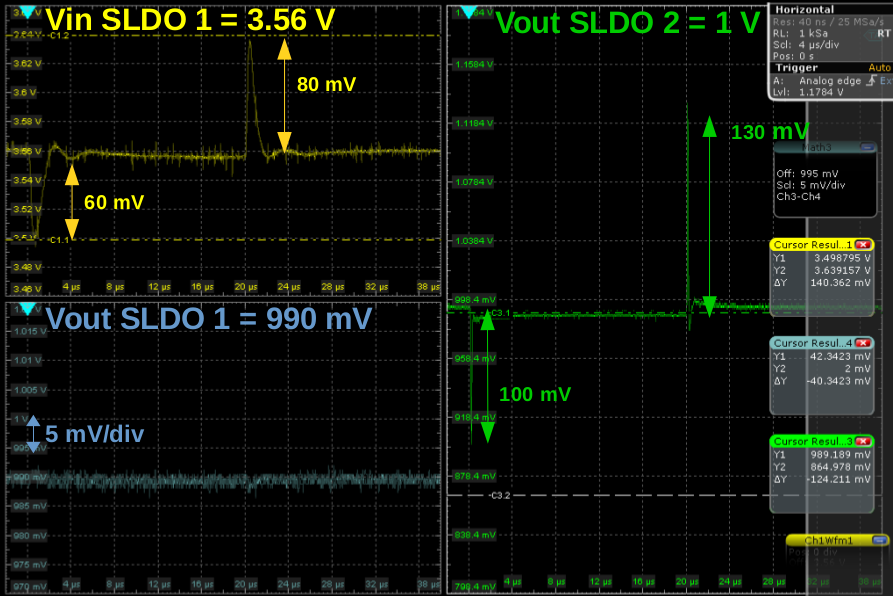
\includegraphics[scale=.32]{Immagini/ScreenSerie}
\caption{Schermata dell'oscilloscopio in cui è riportata in giallo la tensione in ingresso al primo ShuntLDO della catena,  in celeste la tensione di $\mathrm{V_{out}}$ sempre dello ShuntLDO1 e in verde la tensione di $\mathrm{V_{out}}$ dello ShuntLDO2 su cui è applicato il carico dinamico. Le fluttuazioni in tensione originate dalla variazione di carico sullo ShuntLDO2 si ripercuotono sul $\mathrm{V_{in}}$ dello ShuntLDO1 (giallo) ma non sulla tensione da esso generata (celeste).}
\label{ScreenSerie}
\end{figure}
In verde è riportato l'andamento di $\mathrm{V_{out}}$ del secondo ShuntLDO, che mostra importanti undershoot e overshoot, i quali, a loro volta e come visto in precedenza, causano come visto in precedenza, fluttuazioni della tensione in ingresso. 
La tensione di ingresso dello ShuntLDO2 corrisponde alla terra della scheda di test su cui si trova lo ShuntLDO1.
Le visibili fluttuazioni di questa, quindi, si ripercuotono su ShuntLDO2.
Nonostante ciò, come risultato importante, si può notare che $\mathrm{V_{out}}$ del primo ShuntLDO sia indipendente da queste.
